
\chapter{Related Work}

\section{Emotion representation}
A still widely-discussed research question in Emotion Recognition is the question about how to best represent emotions, or how to model affect. \citet{Gunes:2011:EmotionRepresentationContinuous} stated that current approaches stem from research in psychology, which distinguishes between three major approaches: \textbf{categorical, dimensional, and appraisal-based.}
% According to research in psychology, three major approaches to affect modelling can be distinguished [1]: categorical, dimensional and appraisal-based approach. The categorical approach claims that there exist a small number of emotions that are basic, hard-wired in our brain and recognised universally (e.g., [2]). This theory on universality and interpretation of affective nonverbal expressions in terms of basic emotion categories has been the most commonly adopted approach in research on automatic measurement of human affect.
% \citep{Gunes:2011:EmotionRepresentationContinuous}
\newline\newline
The \textbf{categorical approach} classifies emotions into a small number of discrete categories, universally-recognised. In this approach, there are six or seven categories, namely, 'happy', 'sad', 'fear', 'anger', 'disgust', 'surprise' and sometimes also 'neutral' \citep{Hupont:2010:FacialEmotionsIn2DAffectiveSpace}. Even though there are many other ways to represent emotions, \citet{Salah:2018:VideoBasedER} argued that this approach is still very relevant today, as it is more natural for humans to interpret emotions in that way. This was supported by \citet{Gunes:2011:EmotionRepresentationContinuous} who posited that the theory on universality, as well as the facility of interpretation has made this approach the most commonly adopted in research on automatic measurement of human affect.
\newline\newline
However, \citet{Gunes:2011:EmotionRepresentationContinuous} argued that this categorical approach is not able to capture the complexity of the affective state exhibited by people in complex and subtle ways (e.g., embarrassment).
% However, a number of researchers have shown that in everyday interactions people exhibit non-basic, subtle and rather complex affective states like thinking, embarrassment or depression. Such subtle and complex affective states can be expressed via dozens of anatomically possible facial and bodily expressions, audio or physiological signals. Therefore, a single label (or any small number of discrete classes) may not reflect the complexity of the affective state conveyed by such rich sources of information
% \citep{Gunes:2011:EmotionRepresentationContinuous}
\newline\newline
%The most widely used dimensional model is a circular configuration called Circumplex of Affect introduced by Russell [3]. This model is based on the hypothesis that each basic emotion represents a bipolar entity being a part of the same emotional continuum. The proposed polars are arousal (relaxed vs. aroused) and valence (pleasant vs. unpleasant)
% \citep{Gunes:2011:EmotionRepresentationContinuous}
\citet{Hupont:2010:FacialEmotionsIn2DAffectiveSpace} proposed a widely-used dimensional approach called 'Continuous Affective Space'. Instead of representing emotions in discrete categories, the Continuous Affective Space approach represented emotions as a point in a two-dimensional plane. This approach allowed for the representation of emotion as a combination of two values: valence and arousal. Valence indicates how positive or negative an emotion was, while arousal indicates how calming or exciting an emotion was \citet{Hupont:2010:FacialEmotionsIn2DAffectiveSpace} claim that this approach allowed them to capture more information by considering intermediate emotional states.
% Hupont, Cerezo, and Baldassarri(2010): Continous Affective Space, mapping emotions into a 2D space allowing them to consider intermediate emotional states (intermediate emotional state = in-between emotions, gradients of emotions e.g., anxiety to fear, horror to disgust [presumably]). This study allowed for the representation of emotions as a point in a plane, instead of mere items in a categorical list.
% Valence (whether emotion is + or -), arousal (strength of the emotion of expression)
% \citep{Hupont:2010:FacialEmotionsIn2DAffectiveSpace}
\newline\newline
However, \citet{Salah:2018:VideoBasedER} objected that it is possible for a complex emotion to be reduced to a point in a valence-arousal region. She used ’love’ to exemplify that positive or negative values can be attributed to an emotion, depending on the context. While 'love' can usually be identified with a positive valence, a concerned expression of a mother looking at her sick child could be mapped to a negative valence. Therefore, \citet{Salah:2018:VideoBasedER} argued that there was still a need to map such points to a semantic space in order for humans to properly interpret the emotion.
% However, categorical and discrete approaches that go beyond the six (or seven, if we include “contempt”) basic expressions are still very relevant, as their interpretation is more natural for humans. Also, it is difficult to reduce a complex emotion to a point or region in the valence-arousal space. For instance, we can claim that “love” is a positive emotion, and has a positive valence, but this is not always the case. Consider the loving, concerned expression of a mother, looking at her sick child, and this becomes obvious. Subsequently, a given image or video can be annotated in the continuous space, but there is still a need for mapping such points to a semantic space, where it can be properly interpreted 
% \citep{Salah:2018:VideoBasedER}
\newline\newline
There are entirely different approaches arguing that the two dimensional affective space is insufficient for representing the variety of emotions accurately. Two such approaches are the Pleasure, Arousal and Dominance (PAD) approach \citep{Gunes:2011:EmotionRepresentationContinuous} and the Valence, Arousal and Dominance (VAD) approach \citep{Verma:2017:3D-VAD}
% Another well-accepted and commonly used dimensional description is the 3D emotional space of pleasure – displeasure, arousal – nonarousal and dominance – submissiveness [4], at times referred to as the PAD emotion space [6] or as emotional primitives [7]
% \citep{Gunes:2011:EmotionRepresentationContinuous}
% The valence-arousal model is insufficient to represent emotions accurately. Thus, they introduce a 3D model, called Valence-Arousal-Dominance.
% \citep{Verma:2017:3D-VAD}
\newline\newline
\citet{Gunes:2011:EmotionRepresentationContinuous} pointed out that a major challenge for utilizing affective data is the annotation process, as there existed no general annotation scheme agreed upon by all researchers. Therefore, it cannot be excluded that the annotations possess a personal biases that lean towards the human annotator's personal context and cultural background. Developing an unbiased annotation scheme poses a difficult challenge in practice, as it would need to be unambiguous and facilitate inter-observer agreement.
% A major challenge in affective data annotation is the fact that there is no coding scheme that is agreed upon and used by all researchers in the field that can accommodate all possible communicative cues and modalities. Development of an easy to use, unambiguous and intuitive annotation scheme that is able to incorporate inter-observer agreement levels will indeed ease the heavy burden of the annotation task. Obtaining high inter-observer agreement is another challenge in affect data annotation, especially when (continuous) dimensional approach is adopted.
% \citep{Gunes:2011:EmotionRepresentationContinuous}
\newline\newline
The \textbf{appraisal-based approach} was still considered by \citet{Gunes:2011:EmotionRepresentationContinuous} as an open research question for automatic measurement of affect. The approach consisted of generating emotions through continuous subjective evaluation of the subject's internal state and the state of the outside world.
% In the appraisal-based approach emotions are generated through continuous, recursive subjective evaluation of both our own internal state and the state of the outside world (relevant concerns/needs) [1], [5], [8], [10]. Despite pioneering efforts of Scherer and colleagues (e.g., [11]), how to use the appraisal-based approach for automatic measurement of affect is an open research question as this approach requires complex, multicomponential and sophisticated measurements of change.
% \citep{Gunes:2011:EmotionRepresentationContinuous}


%%%%%%%%%%%%%%%%%%%%%%%%%%%%%%%%%%%%%%%%%%%%%%%%%%%%%%%%%%%%%%%%%%

\section{Emotion Recognition}

\begin{quote}
    Emotion recognition refers in psychology to the attribution of emotional states based on the observation of visual and auditory nonverbal cues. \citep[~p. 3935]{Baenziger:2014:MeasuringERAbility}
\end{quote}
In Computer Science, however, researchers often directly equate facial expressions with peoples emotions. \citet{Barrett:2019:EmotionalFromFacialMovements} claimed that upon a closer examination of existing psychological research, directly tying facial expressions to emotions is unfounded. This is especially true for the categorical approach of emotion representation, as it favors human interpretability over precision. Therefore, the categorical approach assumes that only six or seven basic emotions exist which can be classified by the observation of visual and auditory nonverbal cues.
\newline\newline
It has to be pointed out, however, that even the methods utilized by the researcher in Master's thesis (i.e., looking exclusively at facial expressions, utilizing the AFEW-VA dataset with its annotations) assumed an inherent stance that facial expressions correspond to a person’s emotions. This raises the following question: how much of a person's facial expression corresponds to actual emotions?
\newline\newline
\citet{Barrett:2019:EmotionalFromFacialMovements} admitted that scientific evidence confirms that people do sometimes smile when happy, frown when sad, or scowl when angry. This is true for more cases than assigning discrete emotion categories by chance. The authors clarified that people scowl, on average, less than 30 percent of the time when they are angry. Conversely, 70 percent of the time people do not even scowl when they are angry. Hence, scowls are only one of many expressions of anger. Assuming that anger is only detected when a person scowls, the detection rate is around 30 percent, which is really low. It is even lower when considering that not every scowl implies the emotion of anger. This is backed up by \citet{Barrett:2019:EmotionalFromFacialMovements} when they stated that similar facial movements can express multiple instances of different emotion categories.
% The available scientific evidence suggests that people do sometimes smile when happy, frown when sad, scowl when angry, and so on, as proposed by the common view, more than what would be expected by chance.
% People, on average, the data show, scowl less than 30 percent of the time when they’re angry,” says Barrett. “So scowls are not the expression of anger; they’re an expression of anger — one among many. That means that more than 70 percent of the time, people do not scowl when they’re angry. And on top of that, they scowl often when they’re not angry.”
\newline\newline
Furthermore, facial expressions are interpreted differently by various cultures. \citet{Salah:2018:VideoBasedER} stated that in order to establish a ground truth for a facial expression, the cultural background of the subject and the annotator are needed. If there are two annotators from two different cultural backgrounds, the ratings may differ substantially from each other. The authors \citep{Salah:2018:VideoBasedER} cited an experiment with American and Japanese subjects that were asked to annotate facial expression. Even with a closed set of discrete labels the agreement rate was as low as 54.5\% for "fear" and 64.2\% for "anger" annotations. These results proved the existence of a strong annotator bias in every dataset. However, \citet{Salah:2018:VideoBasedER}, whether this is good or bad depended on whether we want the application's algorithm to learn that bias.
% For emotion estimation, we have ample empirical evidence that different cultures interpret facial expressions differently [39]. According to these findings, establishing ground truth for a facial expression database requires the annotation of both the subject and the annotator’s cultural background. If the same database is annotated by, say, Japanese and American subjects, we may get different ratings, unless a very clear, discrete categorization is used. The typical scenario of letting the annotators choose from a closed set of annotation labels may mask the differences in perception, and even when a closed set is used, we see empirical evidence for these differences. In an early study, Matsumoto indeed experimented with American and Japanese subjects, and obtained as low as 54.5% agreement for “fear” annotations and 64.2% agreement for “anger” annotations in Japanese subjects, even with a closed set of discrete labels for annotation [57]. In any case, we may or may not want the algorithm to learn the biases of the annotators, depending on the application. If an algorithm is pre-screening applicants for a job interview selection decision (a highly undesired situation, but may be conceivable for job posts with tens of thousands of applicants), we do not want any biases there
%\citep{Salah:2018:VideoBasedER}
\newline\newline
\citet{Barrett:2019:EmotionalFromFacialMovements} did not only see differences in respect to facial expression interpretation across cultures, but also across different situations and even across people within a single situation. Because of this, companies and institutions that use AI for Emotion Recognition and base their decisions on these outcomes might inadvertently end up misleading their customers. Therefore, \citet{Barrett:2019:EmotionalFromFacialMovements} were of the opinion that humans need to completely rethink our relationship with emotions, as emotions are varied, complex, and situational. \citet{Barrett:2019:EmotionalFromFacialMovements} compared the needed change in thinking to Charles Darwin's work on the nature of species, as Darwin recognized that each species is a category of highly variable individuals. The same was regarded as true by \citet{Barrett:2019:EmotionalFromFacialMovements} for emotional categories.
% Yet how people communicate anger, disgust, fear, happiness, sadness, and surprise varies substantially across cultures, situations, and even across people within a single situation. 
% \citep{Barrett:2019:EmotionalFromFacialMovements}
% This, in turn, means companies that use AI to evaluate people’s emotions in this way are misleading consumers.
% \citep{Barrett:2019:EmotionalFromFacialMovements}
% Barrett says that perhaps the most important takeaway from the review is that we need to think about emotions in a more complex fashion. The expressions of emotions are varied, complex, and situational. She compares the needed change in thinking to Charles Darwin’s work on the nature of species and how his research overturned a simplistic view of the animal kingdom. “Darwin recognized that the biological category of a species does not have an essence, it’s a category of highly variable individuals,” says Barrett. “Exactly the same thing is true of emotional categories.”
% \citep{Barrett:2019:EmotionalFromFacialMovements}
\newline\newline\newline
\textbf{Technical state-of-the-art}\newline
Despite all the aforementioned considerations about recognizing emotions from facial expressions, researchers are striving to come up with better ways to improve algorithms and their recognition results.
\newline\newline
A notable example is the Facial Action Coding System (FACS) proposed by \citet{Ekman:2002:FACS} which is a way of describing visually discernible facial movements, and is composed of a set of codes, also called Action Units (AUs). These AUs describe the presence and intensity of facial muscle movements. FACS, however, is purely descriptive, it is blind about whether these AUs express any emotions. The descriptive nature of this system can help researchers to better interpret facial expressions.

% In fact, our review of the scientific evidence indicates
% hat very little is known about how and why certain
% acial movements express instances of emotion, par
% cularly at a level of detail sufficient for such conclu
% ions to be used in important, real-world applications.
% \citet{Barrett:2019:EmotionalFromFacialMovements}

% Facial Action Coding System, or FACS (Ekman, Friesen, & Hager, 2002), is a systematic approach to describe what a face looks like when facial muscle movements have occurred. FACS codes describe the presence and intensity of facial movements. FACS is purely descriptive and is therefore agnostic about whether those movements might express emotions or any other mental event.11 Human coders train for many weeks to reliably identify specific movements called action units (AUs). Each AU is hypothesized to correspond to the contraction of a distinct facial muscle or a distinct grouping of muscles that is visible as a specific facial movement.
% \citep{Barrett:2019:EmotionalFromFacialMovements}

Emotion Recognition is always based on the observation of subjects in order to attribute them an emotional state. In an optimal scenario, researchers would be able to observe the subjects' thoughts directly. However, the closest researchers got to observing thoughts, is the observation of brain activity through an EEG analysis. \citet{Xing:2019:EEGAudioVisual} did exactly this experiment: they showed video clips to participants, measured the brain activity and fused those measurements with video and audio data. \citet{Xing:2019:EEGAudioVisual} stated that they were able to achieve their best results through this approach.
\newline
While this approach is very promising, the authors pointed out that there was, at the time, no dataset available that obtains EEG signals about emotion activity from participants through video stimulation. Because an EEG is required to produce such a dataset, it would contain no 'In-the-Wild' specimens. Needless to say, it would be very difficult to apply such models in real-life situations, as an EEG is not readily available in every household.
\newline\newline
Current researchers base their predictions on more information in an effort to focus on improving the expressiveness of their Emotion Recognition models. One of the most common approaches that researchers take is finding the best combination of signal fusion (e.g., audio-video and mouse movements). These signal combinations are often supported with extracted features, which help to efficiently characterize the emotional content of the chosen signals. A way of extracting features from video signals could, for example, be the usage of AUs to describe facial muscle movements. 
\newline\newline
Prior to feature extraction in Emotion Recognition, it is essential to perform face recognition in order to set a bounding box for the person's face. Sometimes the face is recognized by the chosen model architecture at training time, however, when setting a bounding box or detecting landmarks, the facial recognition needs to be performed separately. Nowadays, there are publicly available pre-trained algorithms, like the MTCNN algorithm \citep{Zhang:2016:MTCCN} that perform the task of face recognition, bounding boxing and also landmark detection in one go. As stated by \citet{Zhang:2016:MTCCN}, all these three tasks are somewhat correlated, which is why it makes sense to combine them in one three-layered architecture. The achieved results were better than multiple state-of-the-art architectures from 2016.
% approach: tasks of face detection, bounding boxing and landmark detection are closely related and somehow dependent on each other. Thus they made use of a three layered CNN architecture where they start to detect faces in the first CNN, go over to set the bounding box and then detect the facial landmarks. All this combined in one three-layered architecture, namely MTCNN - Multi-Task Convolutional Neural Network
% This approach delivered significantly better results over multiple state-of-the-art architecture for face detection, alignment and landmark detection from the year 2016.
% \citep{Zhang:2016:MTCCN}
\newline\newline
Combining various signals by fusing them before feeding them into a Machine Learning model is a common trend in Emotion Recognition research. The most obvious choice is to combine audio with visual signals, as was done by \citet{Yan:2016:MultiClueFusion} and \citet{Hossain:2019:AudioVisualER}. \citet{Xing:2019:EEGAudioVisual} combined their visual and audio signals with signals from an EEG analysis. All of them argued that their approach achieved significantly better results than their comparison baseline.\newline
Even though it is currently very common that signal fusion happens with video and audio signals, \citet{Akcay:2020:SpeechEmotionRecognition(SER)} pointed out that audio signals could be combined with a wide variety of signals such as visual signals, physiological signals, linguistic features, mouse movements and keystroke dynamics.


%%%%%%%%%%%%%%%%%%%%%%%%%%%%%%%%%%%%%%%%%%%%%%%%%%%%%%%%%%%%%%%%%%%%%%

\section{Identification of human intentions}
The ultimate intention of this research is, to apply the obtained results from Emotion Recognition in a real-life application. With that goal in mind, the researcher deemed it important to first lay out the existing state-of-the-art studies on the identification of human intentions through the observation of facial expressions. One of the envisioned purposes of the resulting application prototype will be to use Emotion Recognition to support consultants during video calls with customers.
\newline\newline
It is of special interest then, for such an application, to be able to identify human interest. As research is really sparse in that specific area, all the current research related to the identification of human intentions will be presented in the following paragraphs:
\newline\newline
\citet{Dong:2012:UnderstandHumanImplicitIntention} did an experiment where they let participants agree or disagree with a statement. The participants were subjected to an \gls{EEG} analysis in order to measure brain activity. The researchers were able to tell by a person’s brain activity whether they agreed or disagreed with a statement even before the person actually vocalized it. Even though the results were very convincing, such an approach would not  be plausible in a real-life setting. .
\newline\newline
Another interesting approach was taken by \citet{Esser:2018:LandmarkDetection}. He used facial Emotion Recognition to visualize the experience of a patient's pain. He made us of an \gls{AAM} for feature extraction in order to better predict the AUs of a person's face. \citeauthor{Esser:2018:LandmarkDetection} was able to measure pain by determining the presence of specific pain-related AUs in a face.
\newline\newline
Identification of customer satisfaction is another practical application of Emotion Recognition. \citet{Ren:2012:ERforCustomerSatisfaction} ran customers' words and comments through Emotion Recognition in order to predict emotions and measure the customer satisfaction. While the researchers succeeded in showing the viability of measuring customer satisfaction, it has to be pointed out that they were working under the assumption that accurate Emotion Recognition results can be directly translated into customer satisfaction.
% Paper from 2012 used customer words and comments to detect customer satisfaction through Emotion Recognition in this information:
% Using an annotated emotion corpus (Ren-CECps), we
% first present a general evaluation of customer satisfaction
% by comparing the linguistic characteristics of emotional
% expressions of positive and negative attitudes. The associations in four negative emotions are further investigated.
% After that, we build a fine-grained emotion recognition
% system based on machine learning algorithms for measuring customer satisfaction; it can detect and recognize
% multiple emotions using customers’ words or comments.
% The results indicate that blended emotion recognition is
% able to gain rich feedback data from customers, which can
% provide more appropriate follow-up for customer relationship management. \citep{Ren:2012:ERforCustomerSatisfaction}
\newline\newline \citet{Kamaruddin:2016:MeasuringCustomerSatisfaction} took a different approach to identification of customer satisfaction. They predicted emotions from speech signals, and based upon that, they inferred customer satisfaction through a very simple approach: a customer was satisfied if their recognized emotion had a positive value for valence (= a positive emotion), and they were dissatisfied if the value is negative (= a negative emotion).

\begin{figure}[H]
  \begin{center}
  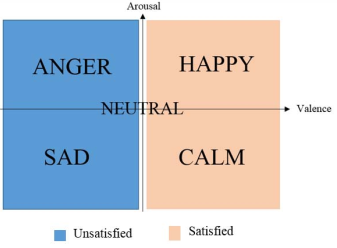
\includegraphics[angle=0, width=0.6\textwidth]{Figures/Satisfaction_from_VA.PNG}
  \caption{Satisfaction inference from VA values}
  \label{fig:SatisfactionFromVA}
  \end{center}
\end{figure}

\citet{Kamaruddin:2016:MeasuringCustomerSatisfaction} realized that using a threshold for defining a 'neutral' region between satisfied and unsatisfied actually performed better in terms of accuracy. However, they admitted that their results were still weak, with 40 \% accuracy for satisfaction determination and 58 \% accuracy for neutral emotion determination.
% In another approach by \citet{Kamaruddin:2016:MeasuringCustomerSatisfaction}, they built upon the hypothesis that the customer is satisfied if he/she is experiencing happiness and neutral emotion whereas if he/she is experiencing sadness or anger, the customer is dissatisfied. They were using Valence and Arousal values and split them up into four emotional values, including one for neutral emotion. They made use of a threshold to define the neutral emotion class. From these classes they directly inferred whether the customer was satisfied or not. Their accuracy stems from the correct prediction of this classes and is with 39 percent accuracy much better than random guessing with 25 percent.
% \begin{quote}
%     We hypothesize that if the valence value is positive (happiness and calm), the customer is satisfied whereas if the valence value is negative (anger and sadness), the customer is not satisfied. Although such approach is simple, it may give us the better understanding of neutral region threshold so that it can be further used for analysis. \citep{Kamaruddin:2016:MeasuringCustomerSatisfaction}
% \end{quote}
\newline\newline
\citet{Poirier:2016:AdsFacialExpression} measured the effectiveness of ads by analyzing facial expressions. \citet{Poirier:2016:AdsFacialExpression} claimed that the emotional journey is the strongest predictor of ad appreciation. The researchers predicted the emotional values for valence and arousal, and focused at the curve/profile created by values for valence. The researchers' assumption seemed to be that a certain profile of the valence curve is the main determinant of whether an ad was successful. While this sounds promising, it also raises the question of whether these ad appreciation in commercial ads also converts into actual positive ratings, or even product sales
% \citet{Poirier:2016:AdsFacialExpression}, the authors measured the effectiveness of ads through facial expressions.
% \begin{quote}
%     emotional journey, which relates to the positive or negative emotional variation  (valence between -1 and 1 where -1: 100\% negative expression, 1: 100\% positive expression and 0: neutral expression), remains the most powerful predictor of ad appreciation 
% \end{quote}
\newline\newline
\citet{Yeasin:2006:MeasurmentOfInterestFromVideo} presented a spatio-temporal approach where they categorized emotions in six classes based on visual data. They mapped those predicted classes to a 3D affect space, and computed the level of interest by calculating L = W x I.  The weight "W" stands for the relative number of images where most motion is concentrated. "I" represents the intensity of an emotion which is calculated by summing up the values for valence, arousal, and stance (3D affect space).
% presents a spatio–temporal approach in recognizing six universal facial expressions from visual data and using them to compute levels of interest. 
% Recognized emotions and used them to calculate a level of interest L, which is calculated as follows: L = W x I. Where I stands for the intensity of an emotion and is calculated through summing up all values from valence, arousal and stance (in a 3D affect space) and mapping these to a range of -5 to +5.
% The weight W is represented by a number in the range of 0 to +1 and measures the relative number of images in a sequence that concentrate most of a motion. The lower the number, the closer the coefficient to 1. \citep{Yeasin:2006:MeasurmentOfInterestFromVideo}



% The FaceReader application \citep{Noldus:2020:Facereader} from Noldus bases their 'Interest' calculation on certain action units instead of recognized emotion values. These action units include:
% \begin{itemize}
%     \item 01 - Inner Brow Raiser
%     \item 02 - Outer Brow Raiser
%     \item 03 - Upper Lid Raiser
%     \item 17 - Chin Raiser
%     \item 20 - Lip Stretcher
%     \item 26 - Jaw Drop
% \end{itemize}
% For the analysis the following time interval is used: Interest - 2 seconds.
